\begin{figure}
  \centering
  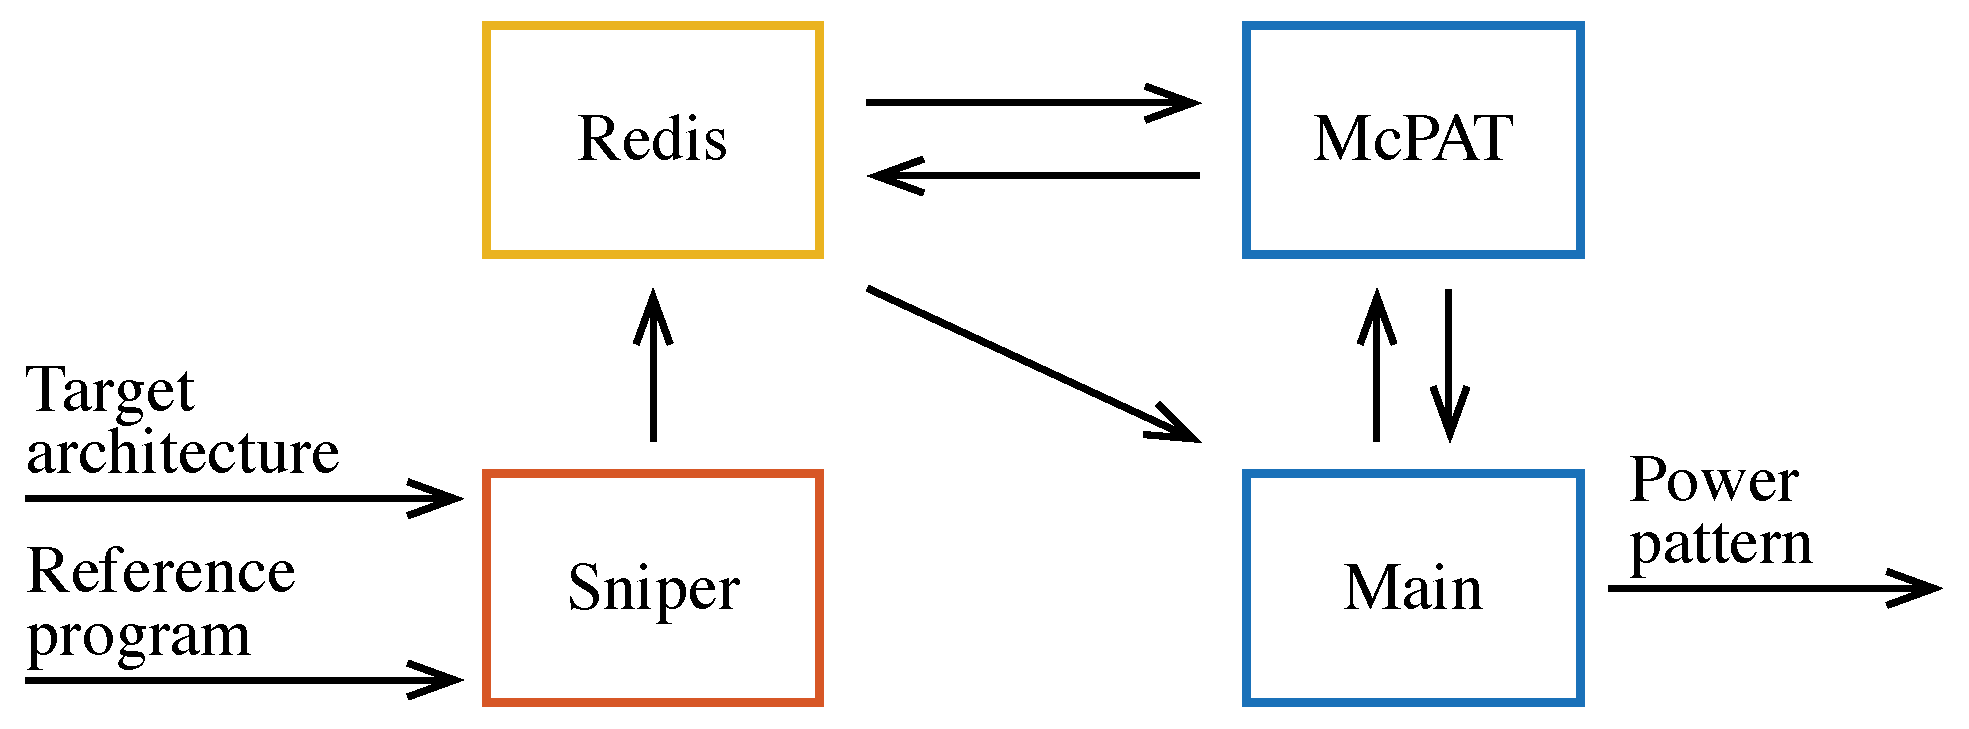
\includegraphics[width=1.0\columnwidth]{include/assets/figures/recorder.pdf}
  \caption{
    The recording infrastructure. The Recorder tool corresponds to the two blue
    boxes on the right-hand side of the figure.
  }
  \flab{recorder}
\end{figure}

The Recorder tool is used at the data-acquisition stage of our methodology. More
specifically, the tool records reference workload patterns, which were discussed
in \sref{workload} and are needed for Streamer. In \fref{methodology}, Recorder
corresponds the bottom-left module with the same name. The tool does not work in
isolation; there is an infrastructure around it. This recording infrastructure
is depicted in \fref{recorder}, in which Recorder itself is given by the two
navy blue modules on the right-hand side.

Given a reference application and a target platform, the starting point is
performance simulation, which we undertake by virtue of the Sniper simulator
\cite{carlson2011}. The output of Sniper is a series of files containing
performance-related information over time. These files are further processed by
our Recorder.

The communications between Sniper and Recorder are handled by Redis (see
\fref{recorder}), which is an in-memory key-value storage commonly used for
caching and message passing. Whenever Sniper produces a new file with
performance information, it sends a message with the file's location to a Redis
queue. Recorder fetches messages from the queue (the diagonal arrow in
\fref{recorder}) and processes the corresponding files. There are several
aspects that are worth noting here. First, the decoupling allows Sniper and
Recorder to work asynchronously, each at its own pace. Second, there can be
multiple Recorder processes serving the same message queue; one only has to
ensure the correct order when storing the data computed by the processes, which
we do. Third, there can be many Sniper processes, each of which simulates a
different program and uses a different queue. The benefit of having a
centralized key-value storage in the last will become clear shortly. The above
aspects make the recording substantially faster.

The next stop is power simulation, which we delegate to \sc{McPAT}
\cite{li2009}. \sc{McPAT} is originally a command-line program; we have made a
shared library out of it and embedded it into Recorder. Hence, power simulation
takes place in the Recorder process, which is emphasized by a color code in
\fref{recorder}. Another important modification that we have made to \sc{McPAT}
is the introduction of a caching mechanism, which was inspired by Sniper. The
caching eliminates repeating certain computations inside \sc{McPAT}, which leads
to considerable time savings. For caching purposes, we use Redis again; see the
arrows between Redis and \sc{McPAT} in \fref{recorder}. All Recorder processes
that are connected to the same Redis server can leverage the same cache, making
the caching mechanism really shine.

Finally, the computed power pattern is stored in a file, which can then be
uploaded to a repository, as described in \sref{workload} and illustrated in
\fref{methodology}. Currently, each output file is an SQLite database
\cite{sqlite}, which implies that the versatile SQL language is automatically at
one's disposal for working with the data.

To summarize, Recorder is used for recording workload patterns. The overall
process can be made substantially faster by launching multiple Sniper processes
along with a single Redis server and multiple Recorder processes.
